\documentclass[11pt, a4paper, english]{article}
\usepackage[margin=1in]{geometry}
\usepackage[utf8]{inputenc}
\usepackage[T1]{fontenc,url}
\usepackage[english]{babel}
\usepackage{textcomp}
\usepackage{amsmath}
\usepackage{verbatim}
\usepackage[hidelinks]{hyperref}
\usepackage{placeins}
\usepackage{frontpage/ifikompendiumforside}
\usepackage{url}
\usepackage[backend=biber]{biblatex}
\usepackage{hyperref}
\usepackage{csquotes}
\usepackage{graphicx}
\graphicspath{{figures/}}
\usepackage{amssymb}
\usepackage{ upgreek }
\usepackage{listings} 



\addbibresource{bibliography.bib}

\title{Frog: Functions for ontologies}
\subtitle{An Essay}
\author{Marlen Jarholt}
\date{19.01.2021} %endre naar ferdig


\lstdefinelanguage{turtle}
{
    columns=fullflexible,
    keywordstyle=\color{red},
    morekeywords={@prefix,@base,@forSome,@forAll,@keywords},
    morecomment=[l]{\#},
    tabsize=4,
    alsoletter={-?}, % allowed in names
    morecomment=[s][\color{blue}]{<}{>},
    basicstyle=\ttfamily\color{black},
    %numberstyle=\color{black},
    morestring=[b][\color{black}]\",
    backgroundcolor=\color{white},
}

\begin{document}

\ififorside

\clearpage

\tableofcontents

\clearpage

%!TEX root = ../master.tex
\section{Functional programaing}

\subsection{(Untyped) Lambda Calculus}
\label{Lambda Calculus}
$\lambda$-calculus is a formal system for expressing computation by Alonzo Church. $\lambda$-calculus consists of terms, binding, and substitution over terms. There are three rules to build up new terms:

\begin{itemize}
    \item \textbf{Variable}: A name which  is a placeholder for a parameter. A variable $x$ is in itself a lambda term.
    \item \textbf{Abstraction}: If we have a term $M$ and an variable $x$, then we also have the term $\lambda x.M$ where $x$ is bound in M.
    \item \textbf{Application}: If $E_1$ and $E_2$ are lambda terms, then $(E_1 E_2) $ is also a lambda term, where $E_2$ is applied to $E_1$.
\end{itemize}

\para
All functions in $\lambda$-calculus are first-class values, which means that a function can take in a function as an argument. Additionally, a function can take another function, or the same function \footnote{Refering the self-application function ($\lambda f.ff$)}, as a return value. Bear in mind that $\lambda$-calculus is left-associative, which means that $E_1 E_2 E_3 \leftrightarrow E_1 (E_2 E_3)$.

\para
In the following sections, refer to \autoref{fig:LC-explenations} for simple visualization of the different parts of a lambda function. 
\begin{figure}
    \centering
    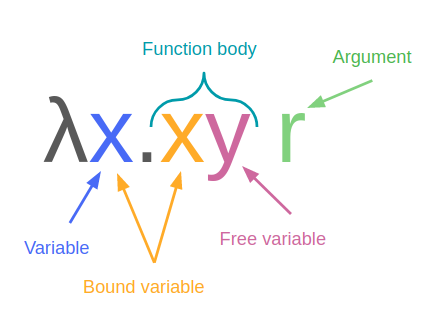
\includegraphics[scale=0.4]{lambdaCalculusFunctionExplenation.png}
    \caption{Visualization of the different parts of a lambda function}
    \label{fig:LC-explenations}
\end{figure}


\subsubsection{Lambda terms}
We have already explained how to build up terms above, but here we provide some extra information to understand terms better. Firstly, the \emph{abstraction} rule is the rule that defines the anonymous function. Secondly, the abstraction only forms the function and binds the variables; the abstraction does not execute the function. 

\subsubsection{Bound and Free variables}
As previously mentioned, the \emph{abstraction} sets the \emph{bound variables}. Within the abstraction, if the variable exists in the function body, the $\lambda$ binds this variable to the function body. For example, given the term $\lambda x.xy$, $x$ is a bound variable because: $x$ occurs in the function body, and $\lambda$ binds $x$ to the function body.

\para
\emph{Free variables} are the opposite of bound variables. Formally, we can say that if we have a term $E_1$ with a set $V_1$ for all variables and $B_1$ for bound variables; 
then the free variables $F_1$ are $F_1 = V_1\setminus B_1$. We can also extend this general rule further, 
by adding another term $E_1$ with a set $V_2$ for all variables and $B_2 $ for all the bound variables;
then the \emph{free variables} in $E_1 E_2$, $F_1 F_2$ equals $ (V_1\setminus B_1) \cup (V_2\setminus B_2)$. 
In other words, the set of free variables in the term $E_1 E_2$ is the union of the free variables in $E_1$ and $E_2$.

\subsubsection{$\alpha$-conversion}
To explain $\alpha$-conversion, one needs to understand what \emph{$\alpha$ equivalence} is. In short, two lambda terms are $\alpha$-equivalent if the only difference in the terms has the variables' names. E.g $\lambda ab.ab$ is alpha-equivalent to the lambda term $\lambda xy.xy$ 

\para
With $\alpha$-equivalent in mind, \emph{$\alpha$-conversion} is a way to change a variable name in both the $\lambda$ part and the function body while keeping the new term $alpha$ equivalent to the old term. E.g. $\alpha$-conversion of $\lambda ab.ab$ is $\lambda xy.xy$ since these are $alpha$ equivalent. Bear in mind that changing a variable name to an already existing variable name in the term is not allowed, because the result would change the meaning and thus the two terms would not be $alpha$ equivalent.

\para
As we have already mentioned, when doing $\alpha$-conversion, we can only change the names of the variables in the term so that the term does not change its meaning. 
E.g., $\lambda x.x \rightarrow_\alpha \lambda y.y$ since we have not changed the meaning of this term. The result of sending in any value/term $e$ will give us the same return value, in this case, just $e$ itself. An example of what is not allowed to do is this $\lambda x.xy \rightarrow_\alpha \lambda y.yy$, as these terms will give us different return values for an argument. Let us try with $e$ again; then we would see that  $\lambda x.xy e$ would give us $ey$ while $\lambda y.yy e$ would give us $ee$, and $ey \neq ee$. So the term $\lambda x.xy$ is $\alpha$-equivalent to all terms where we change to $x$ to anything except $y$. We can generally change any variable name to anything except the set of variables in the function body. Therefore $\lambda x.xy \rightarrow_\alpha \lambda z.zy$. Besides, we need to make sure that we only changes the variables that are in the same abstraction. So the term $\lambda x.\lambda x.x $ is not $\alpha$-equivalent to the 
term $\lambda y.\lambda x.y$, but to for example the terms $\lambda y.\lambda x.x$ or $\lambda x.\lambda y.y$.

\subsubsection{$\beta$-reduction}
$\beta$-reduction is a way to reduce terms. We reduce terms by sending in argument(s) for the bound variables. E.g., if we want to reduce the lambda term $\lambda x. x s$, 
we can $\lambda x. x$  $s \rightarrow _\beta s$ (this is the identity function, which gives us back the argument we gave to the function). We can do $\beta$-reduction in several rounds. When there are no more possible $\beta$-reductions, we say that the term has reached the $\beta$-normal form. \autoref{fig:beta-reduction} shows an example on $\beta$-reduction with a $\lambda$-term of one of the arguments. 

\para
If the term stays the same after one $\beta$-reduction, the term will never terminate. An example of a term that does not terminate while using $\beta$-reduction is the self-application function applied on itself $(\lambda f.ff) \lambda f.ff$.

\paragraph{Complexity}
$\beta$-reduction is not an atomic step; this means that one must locate all occurrences of a bound variable in a term, which can be very time-consuming. In O-notation, this will take $O(n)$ time for a term of length n. Also, storing all of these occurrences may become costly in regards to storage. 

\begin{figure}
    \centering
    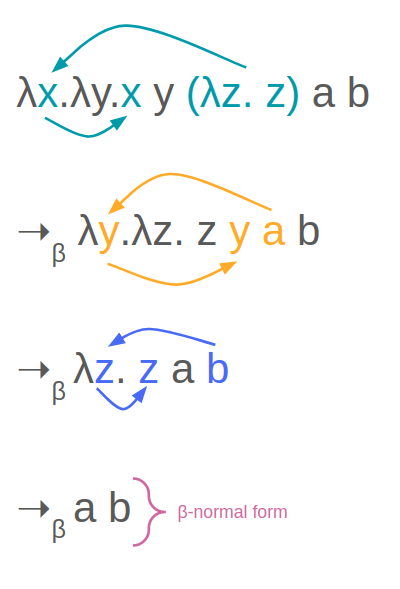
\includegraphics[scale=0.4]{b-reduction.png}
    \caption{An example of $\beta$-reduction}
    \label{fig:beta-reduction}
\end{figure}

\subsubsection{$\eta$-reduction}
$\eta$-reduction is the idea that two functions are equal if, and only if, they return the same result for any given argument. An example of $\eta$-reduction is $(\lambda x.f x)  \rightarrow_\eta f$, whenever $x$ is not a free variable in $f$.

\subsubsection{Combinatory logic}
\label{combinatory logic}
Combinatory logic in computer science, is a theoretical method of computation. The idea is that we only have some base function to create new high-order functions. From now on, these functions will be called primitive functions. These primitive functions combined in the proper order can then express any other high-order function. Combinatory logic is often looked at as a variant of $\lambda$-calculus, where the lambda expressions are replaced with a limited set of primitive functions that does not have any free variables. 
The three primitive functions in combinatory logic is \textbf{I}, \textbf{K} and \textbf{S}.
\\ \\
Where \textbf{I} is the identity function, defined by: \\ 
\begin{center}
    $(I x) = x$\\    
\end{center}
Written in $\lambda$-calculus, the \textbf{I} function would look like this:\\
\begin{center}
    $\lambda x.x$\\    
\end{center}
Futhermore, we have the \textbf{K} function that takes in two arguments and always returns the first argument, defined by:
\begin{center}
    $ ((K x) y) = x$ or $(K x y) = x$\\    
\end{center}
Written in $\lambda$-calculus, the \textbf{K} function would look like this:\\
\begin{center}
    $\lambda xy.x$\\    
\end{center}
Lastly, we have the primitive function \textbf{S}, which takes in three arguments and applies the last argument on the two first arguments:
\begin{center}
    $ (S x y z) = (x z (y z))$\\    
\end{center}
Written in $\lambda$-calculus, the \textbf{S} function would look like this:\\
\begin{center}
    $\lambda xyz.xz(yz)$\\    
\end{center}
From these primitive functions and a variable $x$, we can build up combinatoric terms as shown in \autoref{tab:makeCombinatoricTerms} almost the same way that we build up different terms in $\lambda$-calculs. The difference between combinatoric logic and $\lambda$-calculus, is that we have a limited set of primitive functions in combinatoric logic, and in $\lambda$-calculus we have abstractions.

\begin{table}[]
    \centering
    \begin{tabular}{c c c | c}
         $E :=$&  & $x$ & (variable)\\
         & $|$ & $P$ & (the primitive functions) \\
         & $|$ & $E_1 E_1$ & (application, where $E_1$ and $E_2$ are combinatoric terms)\\
    \end{tabular}
    \caption{How to build up combinatoric terms}
    \label{tab:makeCombinatoricTerms}
\end{table}

\para
If we want to convert a lambda term to an equivalent combinator, we use a transformation $T[]$, which is defined by the following rules:
\begin{enumerate}
    \item $T[x] \Rightarrow x$
    \item $T[(E_1 E_2)] \Rightarrow (T[E_1]\; T[E_2])$
    \item $T[\lambda x.E] \Rightarrow (\textbf{K}\; T[E])$ (if x dosen't occure free in E)
    \item $T[\lambda x.x]\Rightarrow \textbf{I}$
    \item $T[\lambda x. \lambda y.E]\Rightarrow T[\lambda x.T[\lambda y.E]]$ (if x occures free in E)
    \item $T[\lambda x.(E_1 E_2)] \Rightarrow (\textbf{S} \; T[\lambda x.E_1] \; T[\lambda x.E_2])$
\end{enumerate}
T[] is not a well-typed mathematical function but a rewriter, which means that an uncompleted transformation will result in something that is neither a lambda term nor a combinatory term. 

\para
The following example explains how to transform the expression $\lambda x.\lambda y.xy$ from \autoref{fig:beta-reduction}. Note that we have made one shortcut to save time. The shortcut combines rule 3 and 1, which we write as $3/1$ in the example below.
In consequence, $T[\lambda x.y]$ we write $T[\lambda x.y] =_{3/1} (\textbf{K } y)$ instead of $T[\lambda x.y] =_{3} (\textbf{K } T[y]) =_{1} (\textbf{K } y)$.
\begin{quote}
    $\lambda x.\lambda y.xy$ \\
    $=_5 T[\lambda x.T[\lambda y.(xy)]]$ \\
    $=_6 T[\lambda x. (\textbf{S}\; T[\lambda y.x]\; T.[\lambda y.y])]$ \\
    $=_{3/1} T[\lambda x. (\textbf{S}\;(\textbf{K}\; x) \; T.[\lambda y.y])]$ \\  
    $=_4 T[\lambda x. (\textbf{S}\;(\textbf{K}\; x) \; \textbf{I})]$ \\
    $=_6 (\textbf{S} \; T.[\lambda x.(\textbf{S}\;(\textbf{K}\; x))] \; T.[\lambda x.I])$ \\
    $=_{3/1} (\textbf{S} \; T.[\lambda x.(\textbf{S}\;(\textbf{K}\; x))] \; (\textbf{K I}))$ \\
    $=_{6} (\textbf{S} \; (\textbf{S} \; T[\lambda x.\textbf{S}] \; T[\lambda x.(\textbf{K} \; x)]) \; (\textbf{K I}))$ \\
    $=_{3/1} (\textbf{S} \; (\textbf{S} \; (\textbf{K S}) \; T[\lambda x.(\textbf{K} \; x)]) \; (\textbf{K I}))$ \\
    $=_{6} (\textbf{S} \; (\textbf{S} \; (\textbf{K S}) \; (\textbf{S} \; T.[\lambda x.\textbf{K}] \; T.[\lambda x.\textbf{x}]) ) \; (\textbf{K I}))$ \\
    $=_{3/1} (\textbf{S} \; (\textbf{S} \; (\textbf{K S}) \; (\textbf{S} \; (\textbf{K K}) \; T.[\lambda x.\textbf{x}]) ) \; (\textbf{K I}))$ \\
    $=_4 (\textbf{S} \; (\textbf{S} \; (\textbf{K S}) \; (\textbf{S} \; (\textbf{K K}) \; \textbf{I}) ) \; (\textbf{K I}))$ \\      
\end{quote}
It is common to add the combinatory terms \textbf{B} ($(\textbf{C} f g x) = ((f x )g)$) 
and \textbf{C} ($(\textbf{C} f g x) = (f (x g))$). \textbf{C} performes substitution on the the first term, and \textbf{B} on the second term, in contrast to \textbf{S} which performs substitution on both terms. These two terms can now be added to the transformation, $T[]$:
\begin{enumerate}
    \setcounter{enumi}{6}
    \item $T[\lambda x.(E_1 E_2)] \Rightarrow (\textbf{C} \; T[\lambda x.E_1] \; T[E_2]))$ (if x is free in $E_1$ but not in $E_2$)
    \item $T[\lambda x.(E_1 E_2)] \Rightarrow (\textbf{B} \; T[E_1] \; T[\lambda x.E_2])$ (if x is free in $E_2$ but not in $E_1$)
\end{enumerate}
\textbf{B} and \textbf{C} are define as the following using the primitive functions:\\
$\textbf{B=(S(K S)K)}$\\
$\textbf{C=(S(S(K(S(K S)K))S)(K K))}$\\

\subsection{Type theory}
\label{type theory}
Type theory is the academic study of \emph{type systems}, which gives every term a type. The type determines the meaning, and which operations are possible to perform on a term. Lambda Calculus has its own type system, also made by Alonzo Church called \emph{Simply Typed Lambda Calculus}, which we discuss in \autoref{Simply Typed Lambda Calculus}.

\para
\emph{A term} is often followed by a : and then the type of the term. \emph{A type} in a type system is semantically a collection of different values that a term can be evaluated to be. Therefore, there are many similarities between type systems and set theory, although they have their differences. Furthermore, the name of a given term is syntactic. For example, in java, where we have a type that is a collection of all Integers ($\mathbb{Z}$) (semantic) and has the name int (syntactic). Consequently, a term $e$ ($e$ is often used to denote a term) is of type $\tau$ ($\tau$ is often used to denote a type) if $e \in \tau$. E.g. 2 is of type $\mathbb{N}$ (natural numbers) because $2 \in \mathbb{N}$. Making new types depends on the type systems' set of base types and type constructors, often called the \emph{inductive types} of a type system. An example type system with the base type $\sigma$, two type constructors $*$ and $\#$, and two types $M$ and $N$, makes it possible to make a new type $T$ as shown in \autoref{tab:inductive types}. 

\para
Many of the programming languages using type systems either require that all expressions terminate (e.g. Coq) or allow infinite loops but are inconsistent when viewed as logics (e.g. Haskel) \textbf{(src: http://www.tyconmismatch.com/papers/combining-TR.pdf)}.
Therefore in some programming languages like \nameref{Simply Typed Lambda Calculus}, one of the type systems goals is to make sure that a term terminates. 

\begin{table}[]
    \centering
    \begin{tabular}{c c c}
         $T :=$&  & $\sigma$\\
         & $|$ & $M * N$ \\
         & $|$ & $M \# N$ \\
    \end{tabular}
    \caption{Example of how to build up inductive types}
    \label{tab:inductive types}
\end{table}


\subsubsection{Decision problems}
Type theory uses type checking, typability and type inhabitation as decisions problems. These decision problems uses judgments, which are denoted with $\Upgamma \vdash e:\tau$. Where $\Upgamma$ is the denotation which is usually used for a context or environment. A terms' type is determined using the judgment and equivalences type inference rules. 

\para
The decision problem of \textbf{checking} (abbreviated by ($\Upgamma\vdash e : \tau$?) is:\\
\textit{Given a type environment $\Upgamma$, a term $e$, and a type $\tau$, decide whether the term $e$ can be assigned the type $\tau$ in the type environment $\Upgamma$} \\ \\
The decision problem of type \textbf{typability} (abbreviated by ($ \exists \Upgamma,\tau .\Upgamma\vdash e : \tau$?) is: \\ 
\textit{Given  a term $e$, decide wheter there exists a type environment $\Upgamma$ and a type $\tau$ such that the term $e$ can be assigned the type $\tau$ in the type environment $\Upgamma$} \\ \\ 
The decision problem of type \textbf{inhabitation} (abbreviated by ($ \exists e.\Upgamma \vdash e : \tau$?) is: \\
\textit{Given a type environment $\Upgamma$ and a type $\tau$, decide whether there exists a term $e$ that can be assigned the type $\tau$ in the type environment $\Upgamma$}

\subsection{Simply Typed Lambda Calculus}
\label{Simply Typed Lambda Calculus}
As we mention in \autoref{type theory}, Simply Typed Lambda Calculus($\lambda^\rightarrow$) is a Type Theory developed by Alonzo Church for lambda-calculus. In $\lambda^\rightarrow$, we can make types with only one constructor $\rightarrow$ and a set of base types, frequently denoted with a $B$. Thus, we can construct new types from the base types, $B$, combined with constructor $\rightarrow$. Using base types $\tau$ and $\sigma$, for instance, make it possible to construct type $\tau \rightarrow \sigma$. $\tau \rightarrow \sigma$ refers to a function that takes in a term of type $\tau$ and returns a term of type $\sigma$, such as: $\lambda x:\tau. y \; \tau \rightarrow \sigma$. 


\para
The syntax for Simply Typed Lambda Calculus is almost identical to Lambda Calculus, with the difference being that we need to define the variables' type in the abstraction. Simply Typed Lambda Calculus similarly specifies the variables' type as in type theory, with $x:\tau$ for a variable $x$ with type $\tau$. In addition, Simply typed lambda calculus adds a set of term constants for the base types, often denoted with a $c$. \autoref{tab:STLC syntax} shows the complete syntax for Simply Typed Lambda Calculus.


\begin{table}[]
    \centering
    \begin{tabular}{c c c}
         $e :=$&  & $x$\\
         & $|$ & $\lambda x:\tau.M$ \\
         & $|$ &  $M N$ \\
         & $|$ &  $c$ \\
    \end{tabular}
    \caption{Simply Typed Lambda Calculus syntax}
    \label{tab:STLC syntax}
\end{table}

\subsubsection{Typing rules}
Simply Typed Lambda Calculus has four typing rules. To state these rules, Simply Typed Lambda Calculus uses the typing environment we define in \autoref{type theory}. The four typing rules are:

\begin{enumerate}
    \item If we have variable $x$ that is of type $\tau$ in the typing environment $\Upgamma$, then we know that $x$ has type $\tau$.
    \item If we have a constant $c$ of type $T$ in the typing environment $\Upgamma$, then we know that $c$ has type $T$.
    \item If we have a variable $x$ of type $\tau$ in a type environment $\Upgamma$, and a term $e$ of type $\sigma$ in $\Upgamma$; then we have a term $\lambda x\tau .e$ with the type $\tau \rightarrow \sigma$ in $\Upgamma$.
    \item If we have a term $M$ of type $\tau \rightarrow \sigma$ and a term $N$ of type $\tau$ in an typing environment $\Upgamma$; then $M N$ will have the type $\sigma$ in $\Upgamma$.
\end{enumerate}

\subsubsection{Reduction of Simply Typed Lambda Calculus}
Simply Typed Lambda Calculus also uses the $\beta$-reduction and $\eta$-reduction as \autoref{Lambda Calculus} mention. Additionally, the reduction needs to check that the arguments to the function have the right type in typing environment. 

\para
To give an example of $\beta$-reduction, we first need to make a set of the base types. In this case, we only use $Int$, the collection of all-natural numbers. From $Int$, it is possible to make an unlimited set of types, such as $Int$, $Int \rightarrow Int$, $Int \rightarrow Int \rightarrow Int$. For the sake of this example, we add the operation $+$ that adds two numbers together. We use the term $e_1:= \lambda x:Int\: y:Int. + x y:Int \rightarrow Int \rightarrow Int$. The type $Int \rightarrow Int \rightarrow Int$ is a term that takes in an Int and returns a term that takes in an $Int$ and returns an $Int$. Applying $e_2 := 3:Int$ with the third typing rule on the term $e_1$, $e_1 e_2$ results in the term $e_1 e_2$ with the type $Int \rightarrow Int$. This type describes a term that taks in a Int and returns a Int, which we can be prove using $\beta$-reduction on the term:
\\ \\
$e_1 e_2 := (\lambda x:Int\: y:Int. + x y:Int \rightarrow Int \rightarrow Int)\; 3:Int 
\newline\rightarrow_\beta \lambda y:Int. + 3\; y: Int \rightarrow Int$
\\ \\
Again, using the third typing rule and applying $e_3 := 7:Int$ on the term $e_1 e_2:Int \rightarrow Int$ results in the term $e_1 e_2 e_3$ with the type $Int$, proven by $\beta$ reduction: 
\\ \\
$e_1 e_2 e_3 := (\lambda y:Int. + 3\; y: Int \rightarrow Int) \; 7:Int
\newline \rightarrow_\beta + 3:int \; 7:Int = 10$

\subsection{Evaluation strategies}
\emph{Evaluation strategies} are a collection of strategies that decides when a programming language should evaluate an expression. An evaluation strategy chooses, among other things, if the language should evaluate expressions sent into a function before executing the function or send in these expressions and evaluate them at a later stage.

\para
Evaluation strategy has two main strategies \emph{eager evaluation} (strict evaluation) and \emph{non-strict evaluation}. To briefly explain, the eager evaluation evaluates the expression as soon as it is bound, while the non-strict evaluation evaluates the expression as soon as it is utilised.Meaning that eager evaluation evaluates arguments of a function, although these arguments may never be used. Non-strict evaluation can also handle infinite lists, also called streams, because non-strict evaluation only evaluates elements that are used. In this case, the eager evaluation would evaluate forever. Additionally, the eager evaluation evaluates the expression as soon it is bound. Therefore, eager evaluation only evaluates an expression once, regardless of how many times a program utilises it. Non-strict evaluation, on the other hand, ends up evaluating the exact expression n times, where n is how many times the expression is used.

\para
Most Imperative programming languages use eager evaluation because it is easy to avoid unexpected behaviour and conduct debugging compared to non-strict evaluation. It may be challenging to use imperative features like I/O and exception handling when using a non-strict evaluation strategy due to state handling. Although most imperative languages use eager evaluation, they often utilise some non-strict evaluation methods. An excellent example of this is the if-statement. In most languages, the if-statement only evaluates the part of the statement that is true. For instance, the pseudo-code, $if\; a\; then\; b\; else\; c$, will only evaluate $b$ if $a$ evaluates to be true. $c$, on the other hand, will only be evaluated if $a$ is false. However, suppose the if-statement is put into a function and use $a$, $b$, and $c$ as arguments, like $f(a, b,c):= \; if\; a\; then\; b\; else\; c$. In that case, the eager evaluation evaluates all the expressions before running the function; despite that, the programming language only needs to evaluate either $b$ or $c$. While non-strict evaluation, on the other hand, only evaluates the used expressions.

\para
\emph{Lazy evaluation}, also known as call-by-need, is a type of non-strict evaluation often used by functional programming. The result of lazy evaluation being a type of non-strict evaluation is that lazy evaluation evaluates the expression when used. What separates lazy evaluation from the other types of non-strict evaluation, such as call-by-name, is that lazy evaluation also uses memorisation to avoid repeated evaluations.  Memorisation uses a look-up table where the evaluated value of a function for some given arguments is stored.  When lazy evaluation evaluates an expression, it first checks if the expression already exists in the look-up table. If the value exists, lazy evaluation retrieves the value from the table. However, if the value is not present in the look-up table, lazy evaluation evaluates the function to a value and appends this value to the table. 

\para
\autoref{fig:strictVSLazy} is an example of strict evaluation and lazy evaluation with b-reduction. Note the following significant differences between these two approaches in this example:

\begin{itemize}
    \item Strict evaluation evaluates an expression (terms) as soon as it is bound. In contrast, lazy evaluation waits until the expression is used.
    \item Strict evaluation evaluates the expressions (terms) before sending them into the term, while lazy evaluation takes in the whole expression.
    \item On the last two lines in \autoref{fig:strictVSLazy}, lazy evaluation uses memorisation to retrieve the return value rather than evaluating it.
\end{itemize}


\begin{figure}
    \centering
    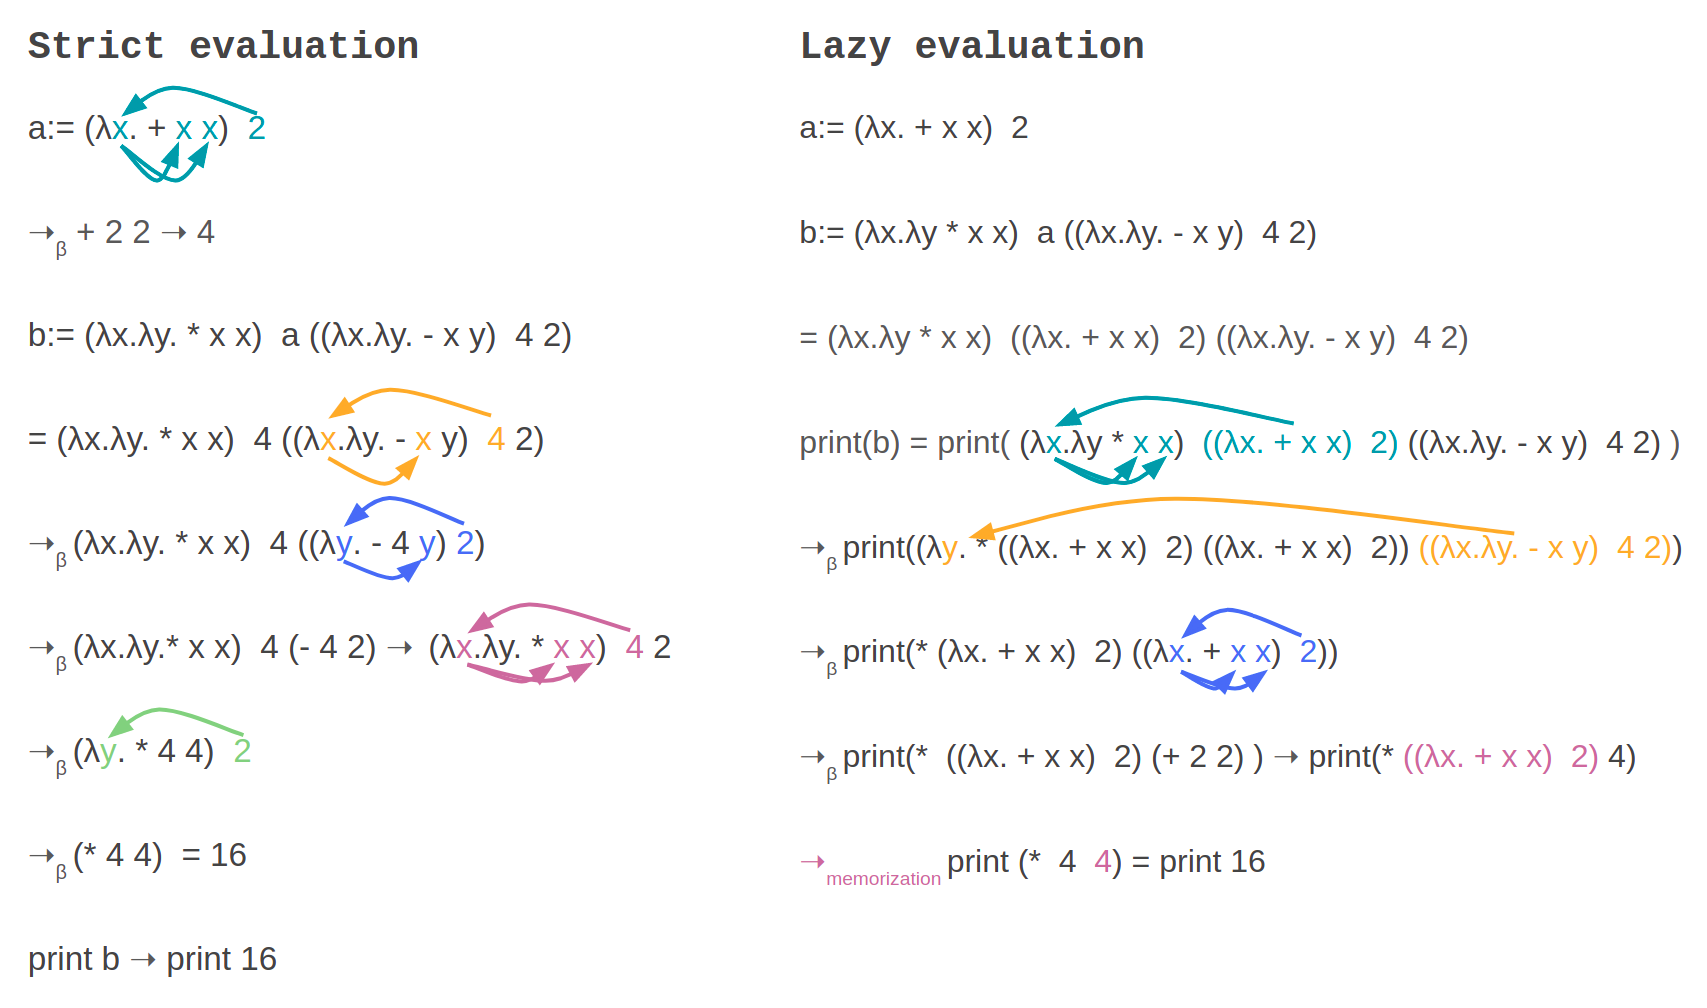
\includegraphics[scale=0.25]{strictVSLazy.png}
    \caption{Shows the difference between strict evaluation and lazy evaluation. Here we assume that print is a term which prints the argument to the terminal, and that +, -, and * are operators that work on integers}
    \label{fig:strictVSLazy}
\end{figure}

\subsection{Practical use of functional programming}
\emph{Functional programming} is a programming paradigm that is made by applying and composing functions. Furthermore, functional programming is inspired by Lambda Calculus definitions. First off, functional programming uses high-order functions, which are functions that can take in functions as arguments and also return a function. In other words, functional programming allows functions to be both an argument and a return value of a function. High-order functions in functional programming enable partial application, also called currying, a technique where every argument to a function is applied sequentially. Partial application applies the function to its argument where each application makes a new function that accepts the next argument.

\para
Some well known high-order functions are map and filter. Map takes a list and a transformation function and returns a new list. Furthermore, map applies the transformation function on each element and adds the result of each transformation to the new list. On the other hand, the filter function takes in a list and a function and applies a subset of the original list to the new list. The filter requires that this transformation function returns a boolean, which indicates if the filter should include the current element in the new list.

\para
Two other important concepts in functional programming are \emph{pure function} and \emph{recursion}. Pure functions are functions without any side effects. The result of using a pure function, among other things, is that the same set of arguments always yields the same return value. A programming language that does not allow any side effects is called a pure programming language. A pure functional programming language will only accept functions without any side effects, resulting in only pure functions. Therefore, it is optimal to use memorisation because we know, as mentioned, that the same set of arguments given to a function always produces the same return value. On the contrary, using memoisation in an impure programming language may be unreliable since it is possible that calling the same function multiple times may not yield the same return value. 

\para
From the 1970s, functional programming started to add type systems in their programming languages, using typed lambda calculus. The reason for using typed lambda calculus is that it makes the program more reliable because it enables compile-time type verification because untyped lambda calculus may yield false-negative errors. 
%!TEX root = ../master.tex
\section{Semantic Web and RDF}
In general semantic web and semantic web technologies is an extension of World Wide Web,
but it dosen't refer to one concrete extension. The goal for the semantic web is to make is to 
make the data that are excesibal on the Internet readable for machine. The main way that the semantic web 
dose this is ot have \textit{linked date} which refers to that the identifiers are pointers to Web addresses 
where we can find more information about hte object.
The data that are conected needs som formal semanitc to work, e.g. RDF, RDFS, OWL etc. These components, shown in figure \nameref{fig:SW stack}
are used to among other things structure the linked data by providing a formal description
of terms, relationships and concept in the knowledge domain. In semanitc web and computer science in general 
we would call this an \textbf{ontologi}, which in short can be defined as the knowledge we have about a given 
domain which is machine-prosecassable and with a formally defined meaning.

\begin{figure}
    \centering
    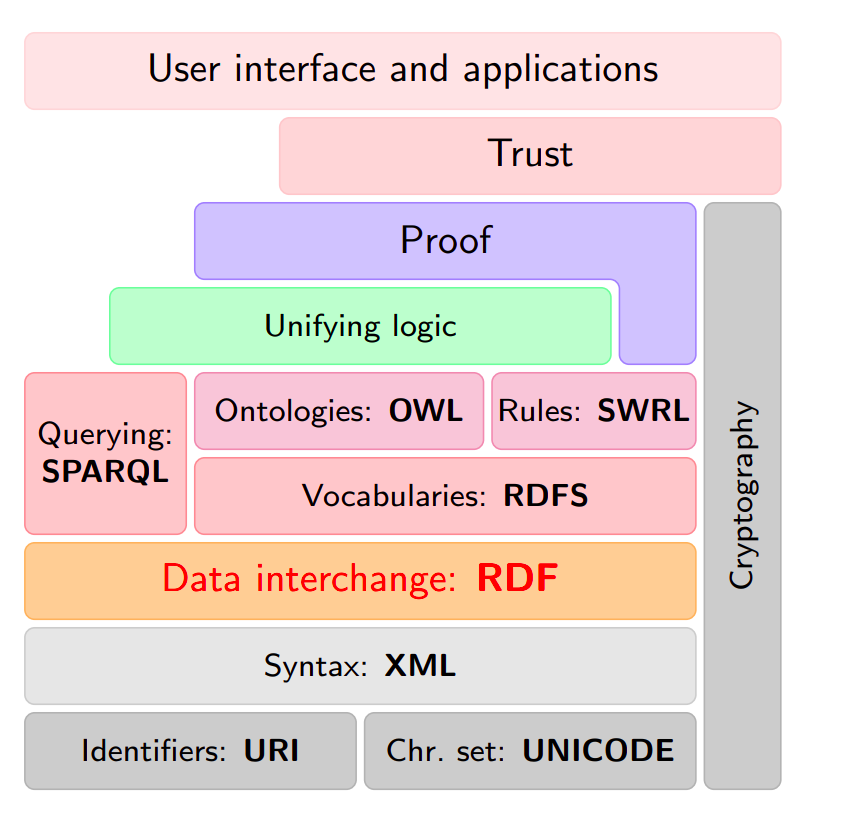
\includegraphics[scale=0.2]{SWStack.png}
    \caption{The semantic web stack src: IN3060 foiler uke 2}
    \label{fig:SW stack}
\end{figure}


\subsection{RDF}
RDF stands for Resource Description Framework and it is a language for formally describing structure data, 
and is the general method in semantic web for describing information that is in a web resource. An RDF document describes 
a directed graph which is build up by tripls which again are build up from subject predicate and object. This is a relation 
from the subject to the object where the predicate tells ous about what the relationship is. In the grap the object 
and subject will be represented as node, with the predicate as an directed edge between the two from the subject to the predicate.
An collection of several will then result in a directed graph. An exampel of an triple can be that Sebastian hasFather Thommas, where 
Sebastian is the object, hasFather is the predicate and Thommas is the object. RDF have several serializations, we will use Turlte for exampels. 
\\ \\
To make this system work we somehow need to uniquely identify the different resources (subject, predicate and objects) of the graph, 
and this is called \textbf{URIs} (Uniform Resource Locators). Every URL is an URI ($URL\subseteq URI$), but it's important to note that 
not all URIs are URL ($URL\nsubseteq URI$). So if we now want to make the tripel made earlier we need to write it out with full URI, that could look 
some thing like this \textit{http://example.org/person/Sebeastian http://example.org/relation/hasFather http://example.org/person/Thommas}
But it can be time consuming to write the whole URI for Sebastian every time we whant to refer to the Sebastian resource, therefore we have something called prefix in 
turtle. We need to set the prefixes in the start of the file with this syntax \textit{@PREFIX ex-p: <http://example.org/person/> .} when we want 
to use the Sebastian resource we can just write $ex-p:Sebastian$. If we now add the the prefix for /relation as well \textit{@PREFIX ex-r: <http://example.org/relation/> .} 
the triple can be written as $ex-p:Sebastian\; ex-r:hasFather\; ex-p:Thommas\; .$.
\\ \\ 
In the ontologi of family, which we have now started to model, it could be nice to express that Sebastian has a father, without us knowing who the father is. 
This can be done with a \textbf{blank node}. In rdf a blank node tells ous that we don't know the URI for the resource, but that we either have some information 
on it or that some other resource is conected to it via a predicate, it is important to note that a blank not can be in the predicate position only in the subject and object
position. So to model that Sebastian has a father we can write either $ex-p:Sebastian\; ex-r:hasFather\; \_:b .$ or $ex-p:Sebastian\; ex-r:hasFather\; [\; ]$ , since the syntax 
for writing an empty node in turtle is either $\_:<some variable name>$ or $[\; ]$. Since an empty node also can be an subject we can express things about the resources. If we 
f.eks. want to model that Sebastian has a father which has a father how is http://example.org/person/Roger we can write $ex-p:Sebastian\; ex-r:hasFather\; [\; ex-r:hasFather\; ex-p:Roger]$
\\ \\ 
In RDF we also have something called literls for expressing stirngs, integer, etc. Literals can only be in the object position of the triple. 
So if we want to express that Sebastian has age 21 we can write $ex-p:Sebastian\; ex-r:hasAge\; " 22 " <opp greie> <opp greie> xsd:int.$ where xsd comes from the prefix
$@prefix\; xsd:\; <http://www.w3.org/2001/XMLSchema\#> .$. We can also model that Sebastian has the name Sebastian in norwiagen and Bastian in english by using 
language tags, this gives use the triples $ex-p:Sebastian\; ex-r:hasName\; Sebastian@no.$ and $ex-p:Sebastian\; ex-r:hasName\; Bastian@en.$. Here har our full 
graph:
\\ \\

\begin{lstlisting}[frame=single, language=turtle]
    @prefix  ex-p:  <http://example.org/person/> . 
    @prefix ex-r:  <http://example.org/relation/> . 
    @prefix xsd: <http://www.w3.org/2001/XMLSchema\#>  . 
    ex-p:Sebastian ex-r:hasFather ex-p:Thommas .
    ex-p:Sebastian ex-r:hasFather [ ex-r:hasFather ex-p:Roger] . 
    ex-p:Sebastian ex-r:hasAge  "22"^^xsd:int . 
    ex-p:Sebastian ex-r:hasName  Sebastian@no . 
    ex-p:Sebastian ex-r:hasName  Bastian@en .
\end{lstlisting}
In addition to the abbreviations we have already made turtle stile have some more abbreviations when writing the triples. For instanse if we have the same 
predicate and subject several times, with different objects, we can just write the predicate and subject one time and seperate the objects with a ,. Futhermore 
we can also abbreviate when we use the same subject severalt times by writne ; in the end of the line instead of . . This gives this turtle file:
\\ \\
\begin{lstlisting}[frame=single, language=turtle]
    @prefix  ex-p:  <http://example.org/person/> . 
    @prefix ex-r:  <http://example.org/relation/> . 
    @prefix xsd: <http://www.w3.org/2001/XMLSchema\#>  . 
    ex-p:Sebastian ex-r:hasFather ex-p:Thommas, [ ex-r:hasFather ex-p:Roger] ; 
                   ex-r:hasAge  "22"^^xsd:int ; 
                   ex-r:hasName  Sebastian@no, Bastian@en ;
\end{lstlisting}

Figure \refname{fig:exampelGraph} is a visual graph of the graph we just made.
\begin{figure}
    \centering
    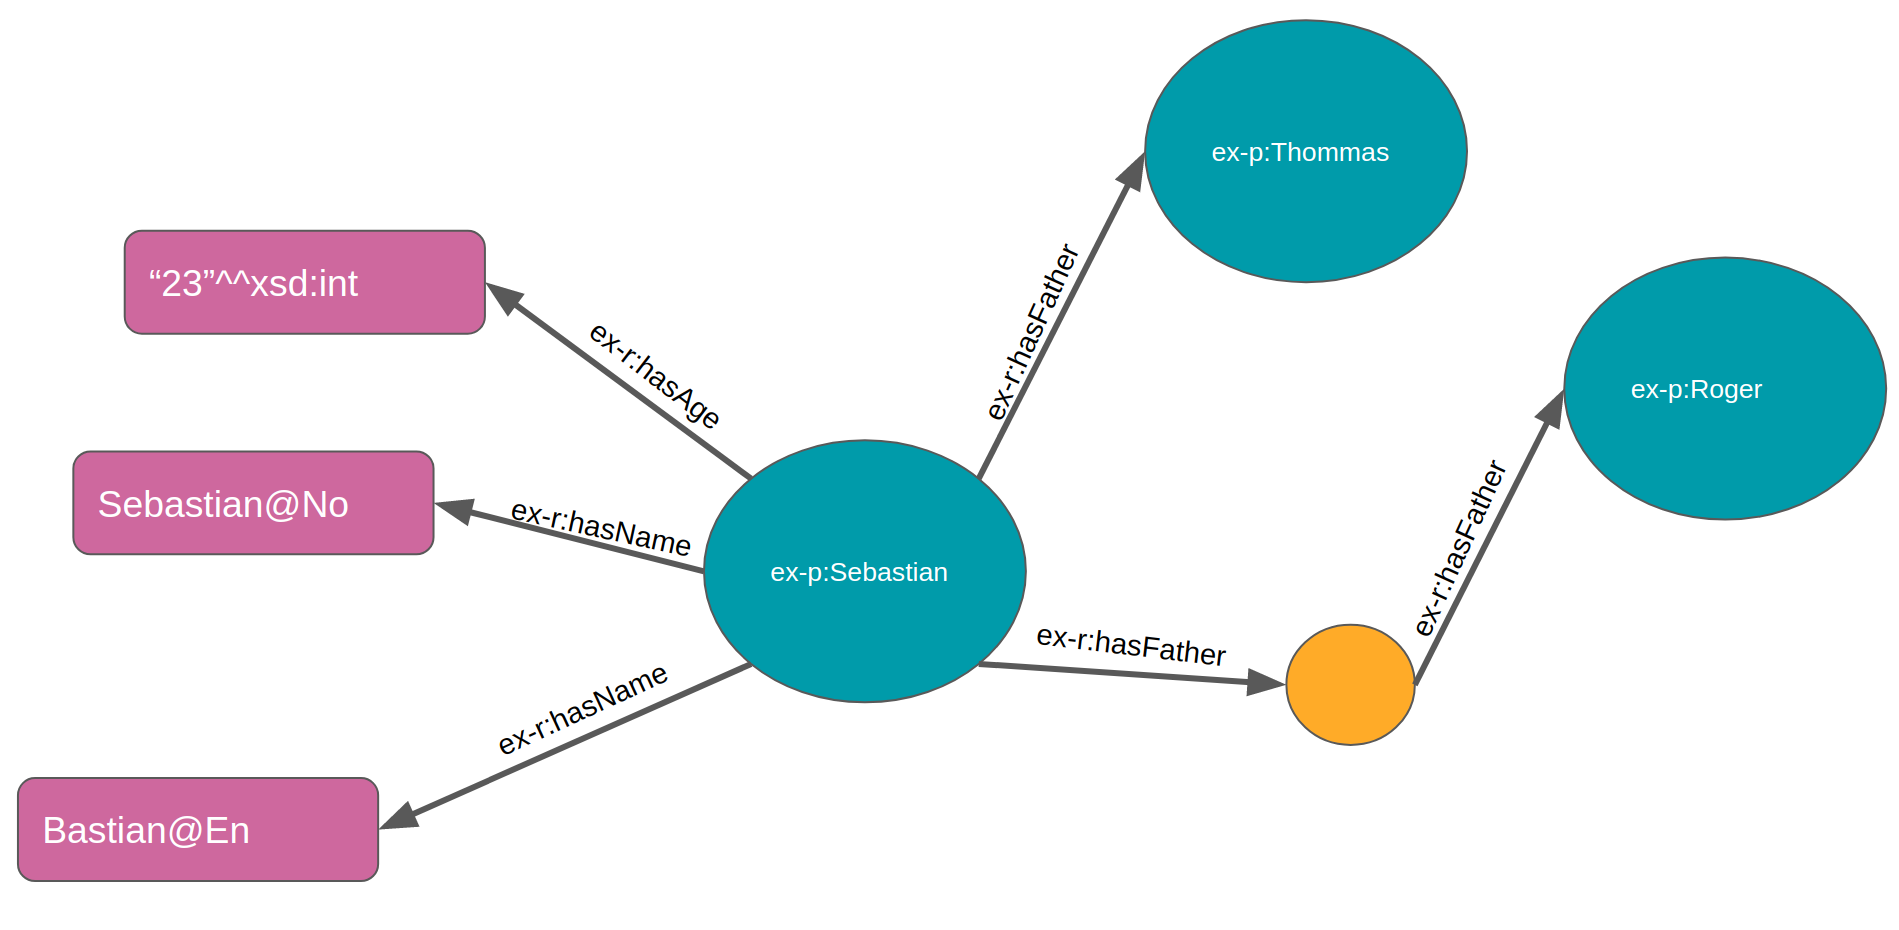
\includegraphics[scale=0.2]{exampleGraph.png}
    \caption{The visual graph over the graph made in section 2.1}
    \label{fig:exampelGraph}
\end{figure}

\subsubsection{Lists in RDF}
In RDF we have two main ways to represent list containers and collections. What is importent to
note is that you can by only using blank nodes as previously mention build up lists, or just
make every individual tripel said in other words the are just abbreviations. Lists in RDF are usually
used when we want to say that a subject have the same relation (or predicate) to several objects.
\\ \\ 
A container has three differents types, namely \textbf{rdf:Seq} (represents an order list), 
\textbf{rdf:Bag} (representing an unordered set) and \textbf{rdf:Alt} (representing a set of alternatives).
A container is build op of a blank node which needs to either have the rdf:type
rdf:Seq, rsd:Bag or rdf:Alt. One important thing to note is that the three different types
don't change (or effects) the structur, only how they will be display them in different applications.
To add nodes we will add a predicate $rdf\_1$ to $rdf\_n$ from the blank node to the member (the name used for 
elements of the container), where the first memeber has ralation $rdf\_1$ and n-th member has relation $rdf\_n$.
So if we whant to add an list to over rdf graph stating all Sebastian ancestors in a unorder set 
it will look like this (Note that we have used the abbreviation \textit{a} for rdf:type):
\begin{lstlisting}[frame=single, language=turtle]
    @prefix  ex-p:  <http://example.org/person/> . 
    @prefix ex-r:  <http://example.org/relation/> . 
    @prefix xsd: <http://www.w3.org/2001/XMLSchema\#>  . 
    @prefix rdf: <http://www.w3.org/1999/02/22-rdf-syntax-ns#> .
    ex-p:Sebastian ex-r:hasFather ex-p:Thommas, [ ex-r:hasFather ex-p:Roger] ; 
                   ex-r:hasAge  "22"^^xsd:int ; 
                   ex-r:hasName  Sebastian@no, Bastian@en ;
                   ex-r:ancestor [a rdf:Bag; 
                                    rdf:_1 ex-p:Thommas; 
                                    rdf:_2 ex-p:Roger].
\end{lstlisting}
The second way to make a list is by using collections. The main differense between a container 
and a collection is that a collection is closed, menaing that we it can't be extended, 
while we can extend a container if we have the reference to the blank node (e.g. \_:list). The reason 
for this is that the linked list is build up like a linked list with \textbf{rdf:first} being a link to the member
and \textbf{rdf:rest} being a link to the rest of the list, when we the have reach the end of the 
list the rdf:rest will link us to \textbf{rdf:nil}. See \nameref{fig:containerAndCollection} to se the 
full structur of the example given above, this figure also shows the differences between the container version
and the collection version. Turlte have an abbreviation for writing collections and that is 
to use () and put all the members of the list insided it. In the general chase it will look like this 
$(member_1 \;member_2 .... member_n)$
To express that all Sebastian ancestors will then look like this:
\begin{lstlisting}[frame=single, language=turtle]
    @prefix  ex-p:  <http://example.org/person/> . 
    @prefix ex-r:  <http://example.org/relation/> . 
    @prefix xsd: <http://www.w3.org/2001/XMLSchema\#>  . 
    @prefix rdf: <http://www.w3.org/1999/02/22-rdf-syntax-ns#> .
    ex-p:Sebastian ex-r:hasFather ex-p:Thommas, [ ex-r:hasFather ex-p:Roger] ; 
                   ex-r:hasAge  "22"^^xsd:int ; 
                   ex-r:hasName  Sebastian@no, Bastian@en ;
                   ex-r:ancestor (ex-p:Thommas rdf:_2 ex-p:Roger).
\end{lstlisting}

\begin{figure}
    \centering
    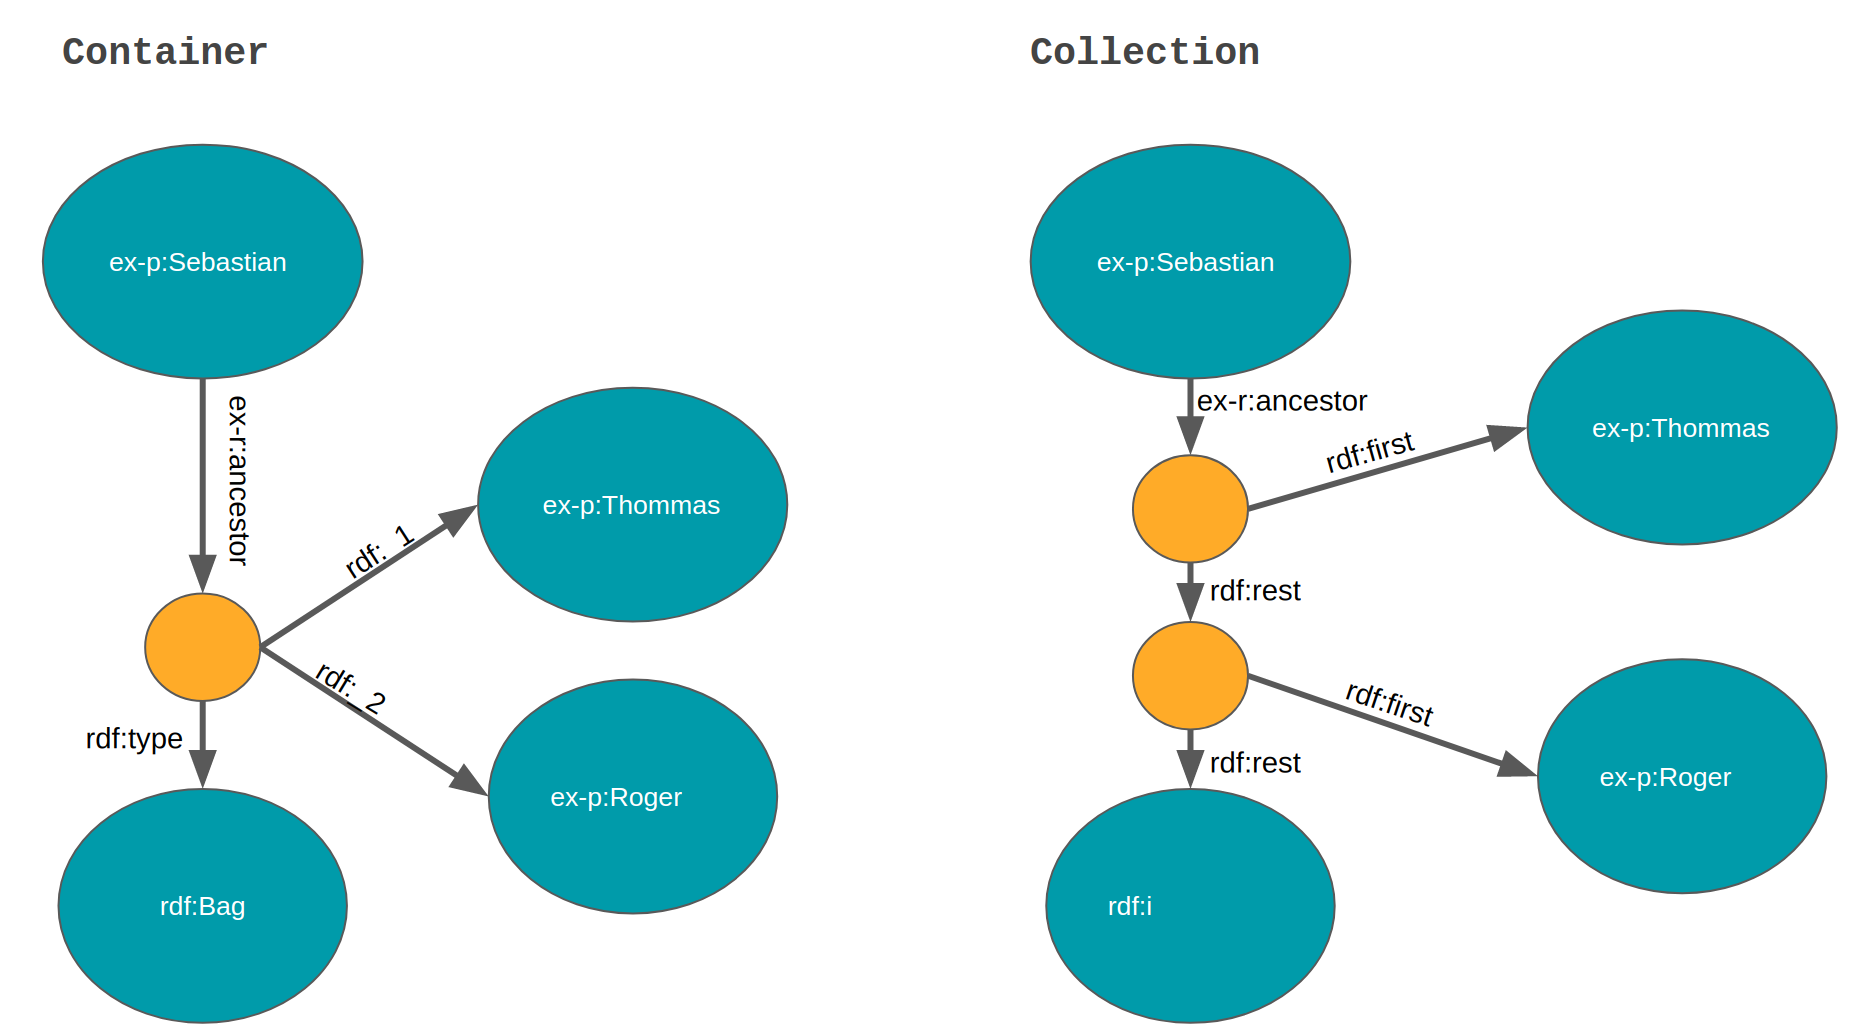
\includegraphics[scale=0.2]{containerAndCollection.png}
    \caption{Shows the difference between a container and a collections in structur}
    \label{fig:containerAndCollection}
\end{figure}

%!TEX root = ../master.tex
\section{Frog}

\subsection{Motivation}
There are no ways change or mainpulate the terms (lists, liters etc) in OTTR. Imagen that you 
make a template for storing information about the weather, you have made sevral hundres instances. Say that one of the 
triples the is made from expanding the template to rdf states somethings temprature in farenheit but you need the temprature in celcius.
For now you how to change the term, meaning that you have to change the degrees manually (or using a scrip) for every OTTR instances.
The goal of Frog is to solve this problem with being a programming language written for OTTR where we are abel to change 
the terms using function. In the farenheit celcius exampel the solution with frog is then to make a function that can be used 
in the template body to convert the farenheit variable given in the head to celcius. 
\\ \\
Having a language like Frog that can make simple functions to mainpulate terms can do more than just convert terms, it can 
also make it possible to add new inffered information. E.g. if we have the template ex-t:Person from earlier
and we want to add a tripel to the expanded template containing the information about whether the person is of type adult (ex-p:Adult) or of type child (ex-p:Child). This 
is information that can be inffered from the age variable, we can make a new rdf-otype with the person as the object, rdf:type as the 
predicate and the result of the function ex-r:ageToLifeStage as the object. Where ex-r:ageToLifeStage is a frog function that takes in an xsd:integer
as argument, and returns a ottr:IRI. The ottr template bellow shows the potential use of the frog function in 
the ex-t:Person.

\begin{lstlisting}[frame=single]
@prefix  ex-p:  <http://example.org/person/> . 
@prefix ex-r:  <http://example.org/relation/> .
@prefix ex-t:  <http://example.org/template/> . 
@prefix ex-f:  <http://example.org/function/> .
@prefix xsd:  <http://www.w3.org/2001/XMLSchema#> . 
@prefix rdf: <http://www.w3.org/1999/02/22-rdf-syntax-ns#> .
@prefix ottr: <http://ns.ottr.xyz/0.4/> .
@prefix o-rdf: <http://tpl.ottr.xyz/rdf/0.1/> .

ex-t:Person [
    ottr:IRI ?person,
    xsd:integer ?age,
    ? List<ottr:IRI> ?fathers,
    ? List<ottr:IRI> ?mothers,
    ? List<ottr:IRI> ?ancestors,
    List<xsd:String> ?names
    ] :: {
    cross | ottr:Triple(?person, ex-r:hasFather, ++?fathers),
    cross | ottr:Triple(?person, ex-r:hasMother, ++?mothers),
    ottr:Triple(?person, ex-r:hasAge, ?age),
    cross | ottr:Triple(?person, ex-r:hasName, ++?names),
    ottr:Triple(?person, ex-r:ancestor, ?ancestors),
    rdf-o:Type(?person, ex-r:ageToLifeStage ?age)
}.
\end{lstlisting}

The expansion the two following two instances

\begin{lstlisting}[frame=single]
ottr:Triple(_:b, ex-r:hasFather, ex-p:Roger) .
ex-t:Person(ex-p:Sebastian, 22 , (ex-p:Thommas, _:b), none, 
(ex-p:Thommas, ex-p:Roger), ("Sebastian"@no, "Bastian"@en)).

ex-t:person(ex-p:Nina, 6, none, none ,none, ("Nina"@no))
\end{lstlisting}

will then be
\begin{lstlisting}[frame=single, language=turtle]
@prefix  ex-p:  <http://example.org/person/> . 
@prefix ex-r:  <http://example.org/relation/> . 
@prefix xsd: <http://www.w3.org/2001/XMLSchema/#>  . 
@prefix rdf: <http://www.w3.org/1999/02/22-rdf-syntax-ns#> .
ex-p:Sebastian ex-r:hasFather ex-p:Thommas, [ ex-r:hasFather ex-p:Roger] ; 
                ex-r:hasAge  "22"^^xsd:int ; 
                ex-r:hasName  "Sebastian"@no, "Bastian"@en ;
                ex-r:ancestor (ex-p:Thommas ex-p:Roger);
                a ex-p:Adult.

ex-p:Nina ex-r:hasAge  "6"^^xsd:int ; 
          ex-r:hasName  "Nina"@no ;
          a ex-p:Child.
\end{lstlisting}

\subsection{Plans for Frog}
The plan is that frog is a language that is written in RDF. In addition to being a high-order functional language, 
with only pure functions. 
Frog will also have a type system, which we will come back to, and it should be clear form the definition of 
the function what the type of the different parameters are and the type of the return value. 
A frog function can only take in arguments and an return values that are a type from the OTTR type system, 
meaning that frog will have the same type system as OTTR.
The advantage of this is that frog can do type checking, since a function has a return value we can check that 
the type of the return value is of the same type that the argument in the instance needs to be.
Since frog is supposed to be a high-order language and will have the same type system as OTTR  
we need to add a new type to the OTTR type system, namely a function type that we need to give to every frog function. 
There is one exception to frog being high-order and that is that a function that is used directly in a 
template (like ex-f:ageToLifeStage in ex-t:Person) aren't allowed to return a function type. Due to addiong a new 
fnction type in the OTTR type system we also need to add terms that maches the new type. 

\subsection{Alternative approaches}
There are several methods that allready exist to add inffered information to rdf graphs, using function or other methods. 
One way you can do this is with SPARQL, which is a query language over RDF with many similarities to SQL for relational 
databases e.g. that they have SELECT, WHERE, GROUP BY, etc, that are build up in a similar fashion. In SPARQL you can use 
a INSERT DATA clause which insert the data in the field in to the graph, combind with a WHERE-clause, and possible a BIND. 
In sparql BIND allows values to be assing to a veriable, meaning that we can make simple functions and bind the result of 
the function to a variable, which again can be used in INSERT DATA clause to add it to the rdf graph. The example that was
described earlier, with converting farenheit to celcius can then be done by using this technique (but here we'll end up with a 
triple with both celcius and farenheit is we don't delete the farenheit afterwards). 
\\ \\
An other alternative to Frog and it's functionalty is OWL. OWL is a Semantic Web language that are made for representing complex 
knowledge, and it's based on logic. In owl we can define the descriptions of classes. Then can use already existing 
predicates and classes to define new ones from inffered information. E.g in the example mention eariler where we defined in the template
with a frog function, wheter the type of the object was child or an adult. This could have been done with modelling in OWL. If we say that  
ex-p:Adult as everthing that has age bigger then 17 and ex-p:Child as everything that has age equal or bigger then 17.
\\ \\
The last method used in the semanitc web we will mention is SWRL, which is a proposed language for semanitc web. SWRL can be used 
to express rules and logic, and is a compination of OWL and a subset of Rule Markup language. SWRL also offers several function 
which can be used on different types (from, rdf, xsd, and owl), but we can not make our own functions, only use the ones that 
SWRL has defined. SWRL is build up with a body that are a set of conditions and a head which is the consequences of the
conditions. Yhe exampel from eariler where we either added the type ex-p:Child or ex-p:Adult can be solved in SWRL with 
making two rules, one for ex-p:Child and one for ex-p:Adult. In the rulte for ex-p:Child we need two condtions on which 
state that the person has an age and one which checks that the age is less than 18 (for this we can use the SWRL function
swrl:lessThan), the conclution of this rule is that the type of the person is ex-p:Child. The ex-p:Adult rule will look 
similar, the conditions will be that the person has an age and that the age is greater then 17 (using the SWRL function 
swrl:greaterThan) and that has the condition that the person has type ex-p:Adult. We can also express the converting from farenheit
to celcius with SWRL using the condition that it has a farenheit temparture and a combination of math functions offerd by SWRL to 
make the conversion as an condition.
\\ \\
The reason it still will be nice to have a language like frog that can be used in the template compared to the 
methodes mention over is that the functions becomes a part of the domain. In additon the methods mention over implies
that we have to add the inffered information before using template. Frog on the other side will offer the abilities to 
do this directly in the template. 
\\ \\
In additon an alternative approache to Frog which is not already meantion and which is not a part of semanitc web 
is using a scripting language to write the functions.
The benefits of making a whole new language like Frog for making functions instead of using a scripting language is 
that is that the types used in frog matches the types in OTTR (in additon to frog doing type checking) meaning that 
the we don't need to transelate types from one type system to another (from the scripting language to OTTR). This means 
that frog probably will be less error-prone than using a scripting language.

\printbibliography

\end{document}